 % methodology part 

% present hardware setup
% Rx side photo : yes
% Tx side photo : on the way 
% discuss synchro methods 
% ? discuss demod ?  => let in appendix ?
% Comparaison and selection


\section{Methodology}
\subsection{Experimental setup}
\begin{frame}
  \only<1>{
  \frametitle{Experimental setup}
  \begin{figure}
    \begin{center}
      \includesvg[width=0.95\textwidth]{figures/layout1.svg}
    \end{center}
    \caption{Setup schematic}
  \end{figure}}

  \only<2>{
  \frametitle{Experimental setup}
  \begin{figure}
    \begin{center}
      \includesvg[width=0.95\textwidth]{figures/layout2.svg}
    \end{center}
    \caption{Setup schematic}
  \end{figure}}


  \only<3>{
  \frametitle{Experimental setup}
  \begin{figure}
    \begin{center}
      \includesvg[width=0.95\textwidth]{figures/layout3.svg}
    \end{center}
    \caption{Setup schematic}
\end{figure}}

  \only<4>{
  \frametitle{Experimental setup}
  \begin{figure}
    \begin{center}
      \includesvg[width=0.95\textwidth]{figures/layout4.svg}
    \end{center}
    \caption{Setup schematic}
  \end{figure}}

\end{frame}


\begin{frame}
  \frametitle{Transmitter side in photo}
  \begin{figure}[ht]
  \begin{adjustwidth}{-10cm}{-10cm}
    \centering
    \begin{subfigure}[ht]{0.5\textwidth}
      \centering
      \includegraphics[width=\textwidth, angle=270]{figures/Tx.jpg}
      \caption{front view}
    \end{subfigure}
    \begin{subfigure}[ht]{0.5\textwidth}
      \centering
      \includegraphics[width=\textwidth, angle=270]{figures/Txpov.jpg}
      \caption{receiver side point of view}
    \end{subfigure}

    \caption{Transmitter side views}
    \end{adjustwidth}
  \end{figure}
\end{frame}


\begin{frame}
  \frametitle{Receiver side in photo}

  \begin{figure}[ht]
  \begin{adjustwidth}{-10cm}{-10cm}
    \centering
    \begin{subfigure}[ht]{0.5\textwidth}
      \centering
      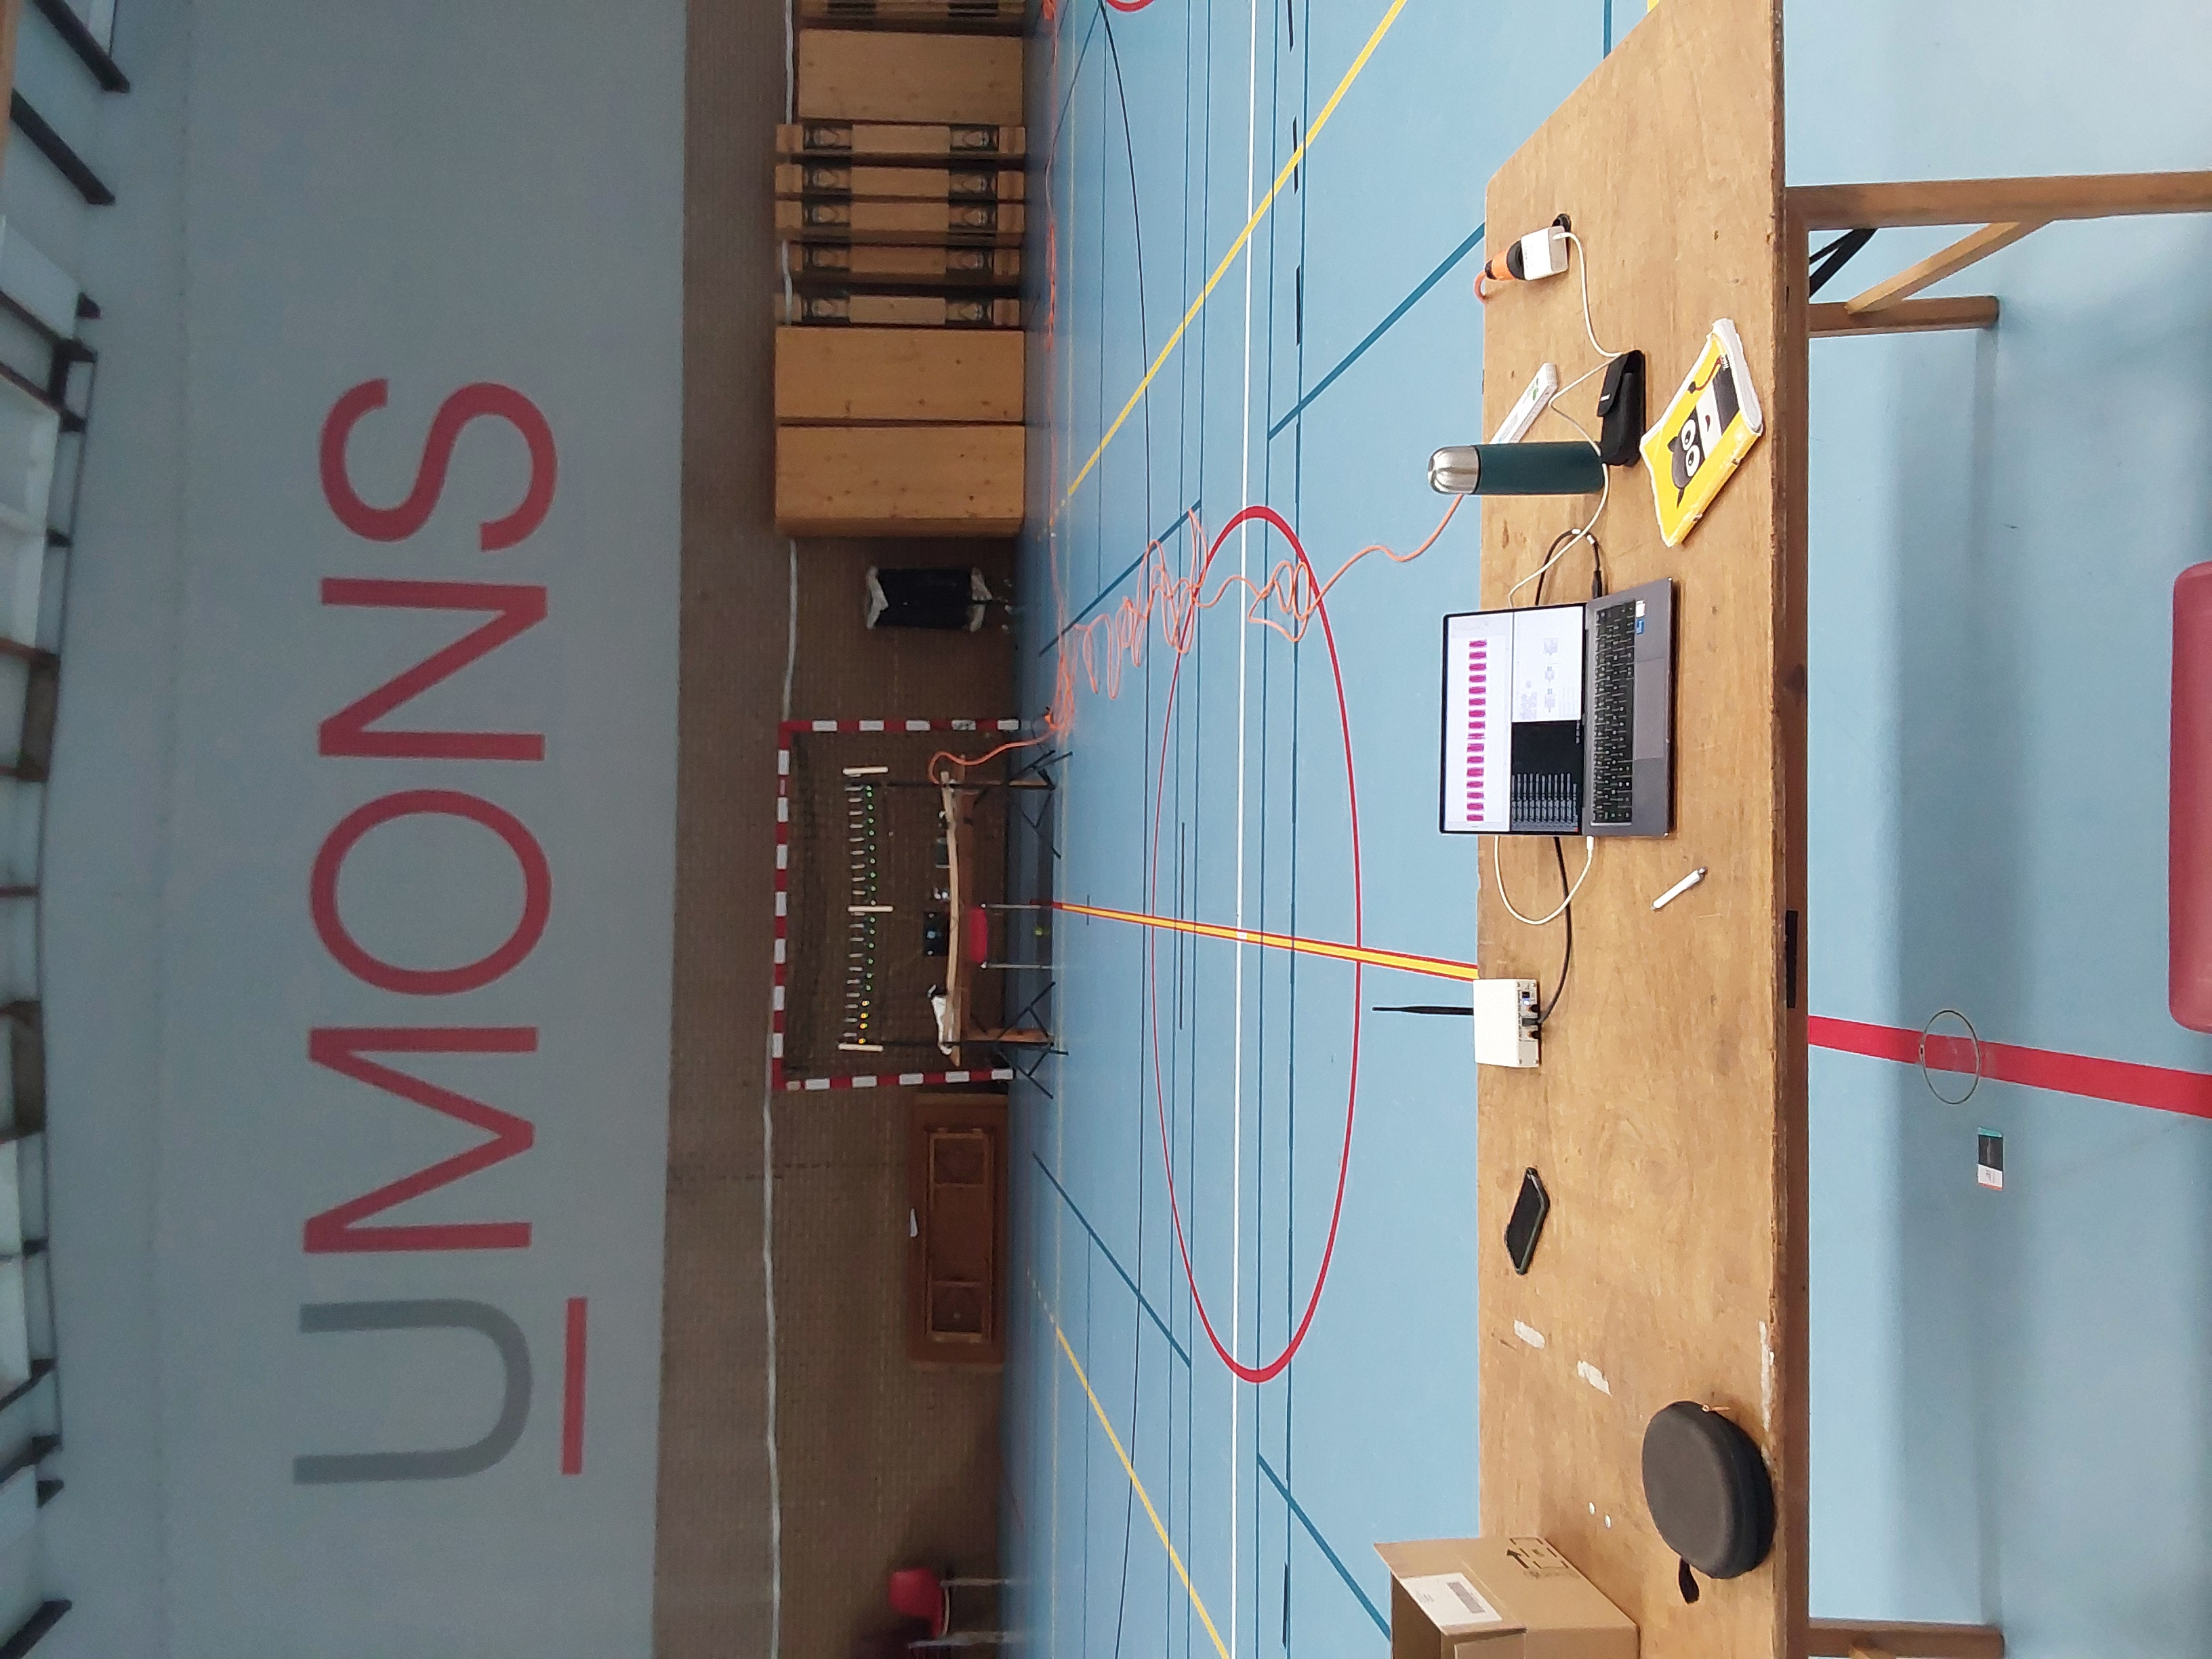
\includegraphics[width=\textwidth, angle=270]{figures/inside rx.jpg}
      \caption{Indoors scenario}
    \end{subfigure}
    \begin{subfigure}[ht]{0.5\textwidth}
      \centering
      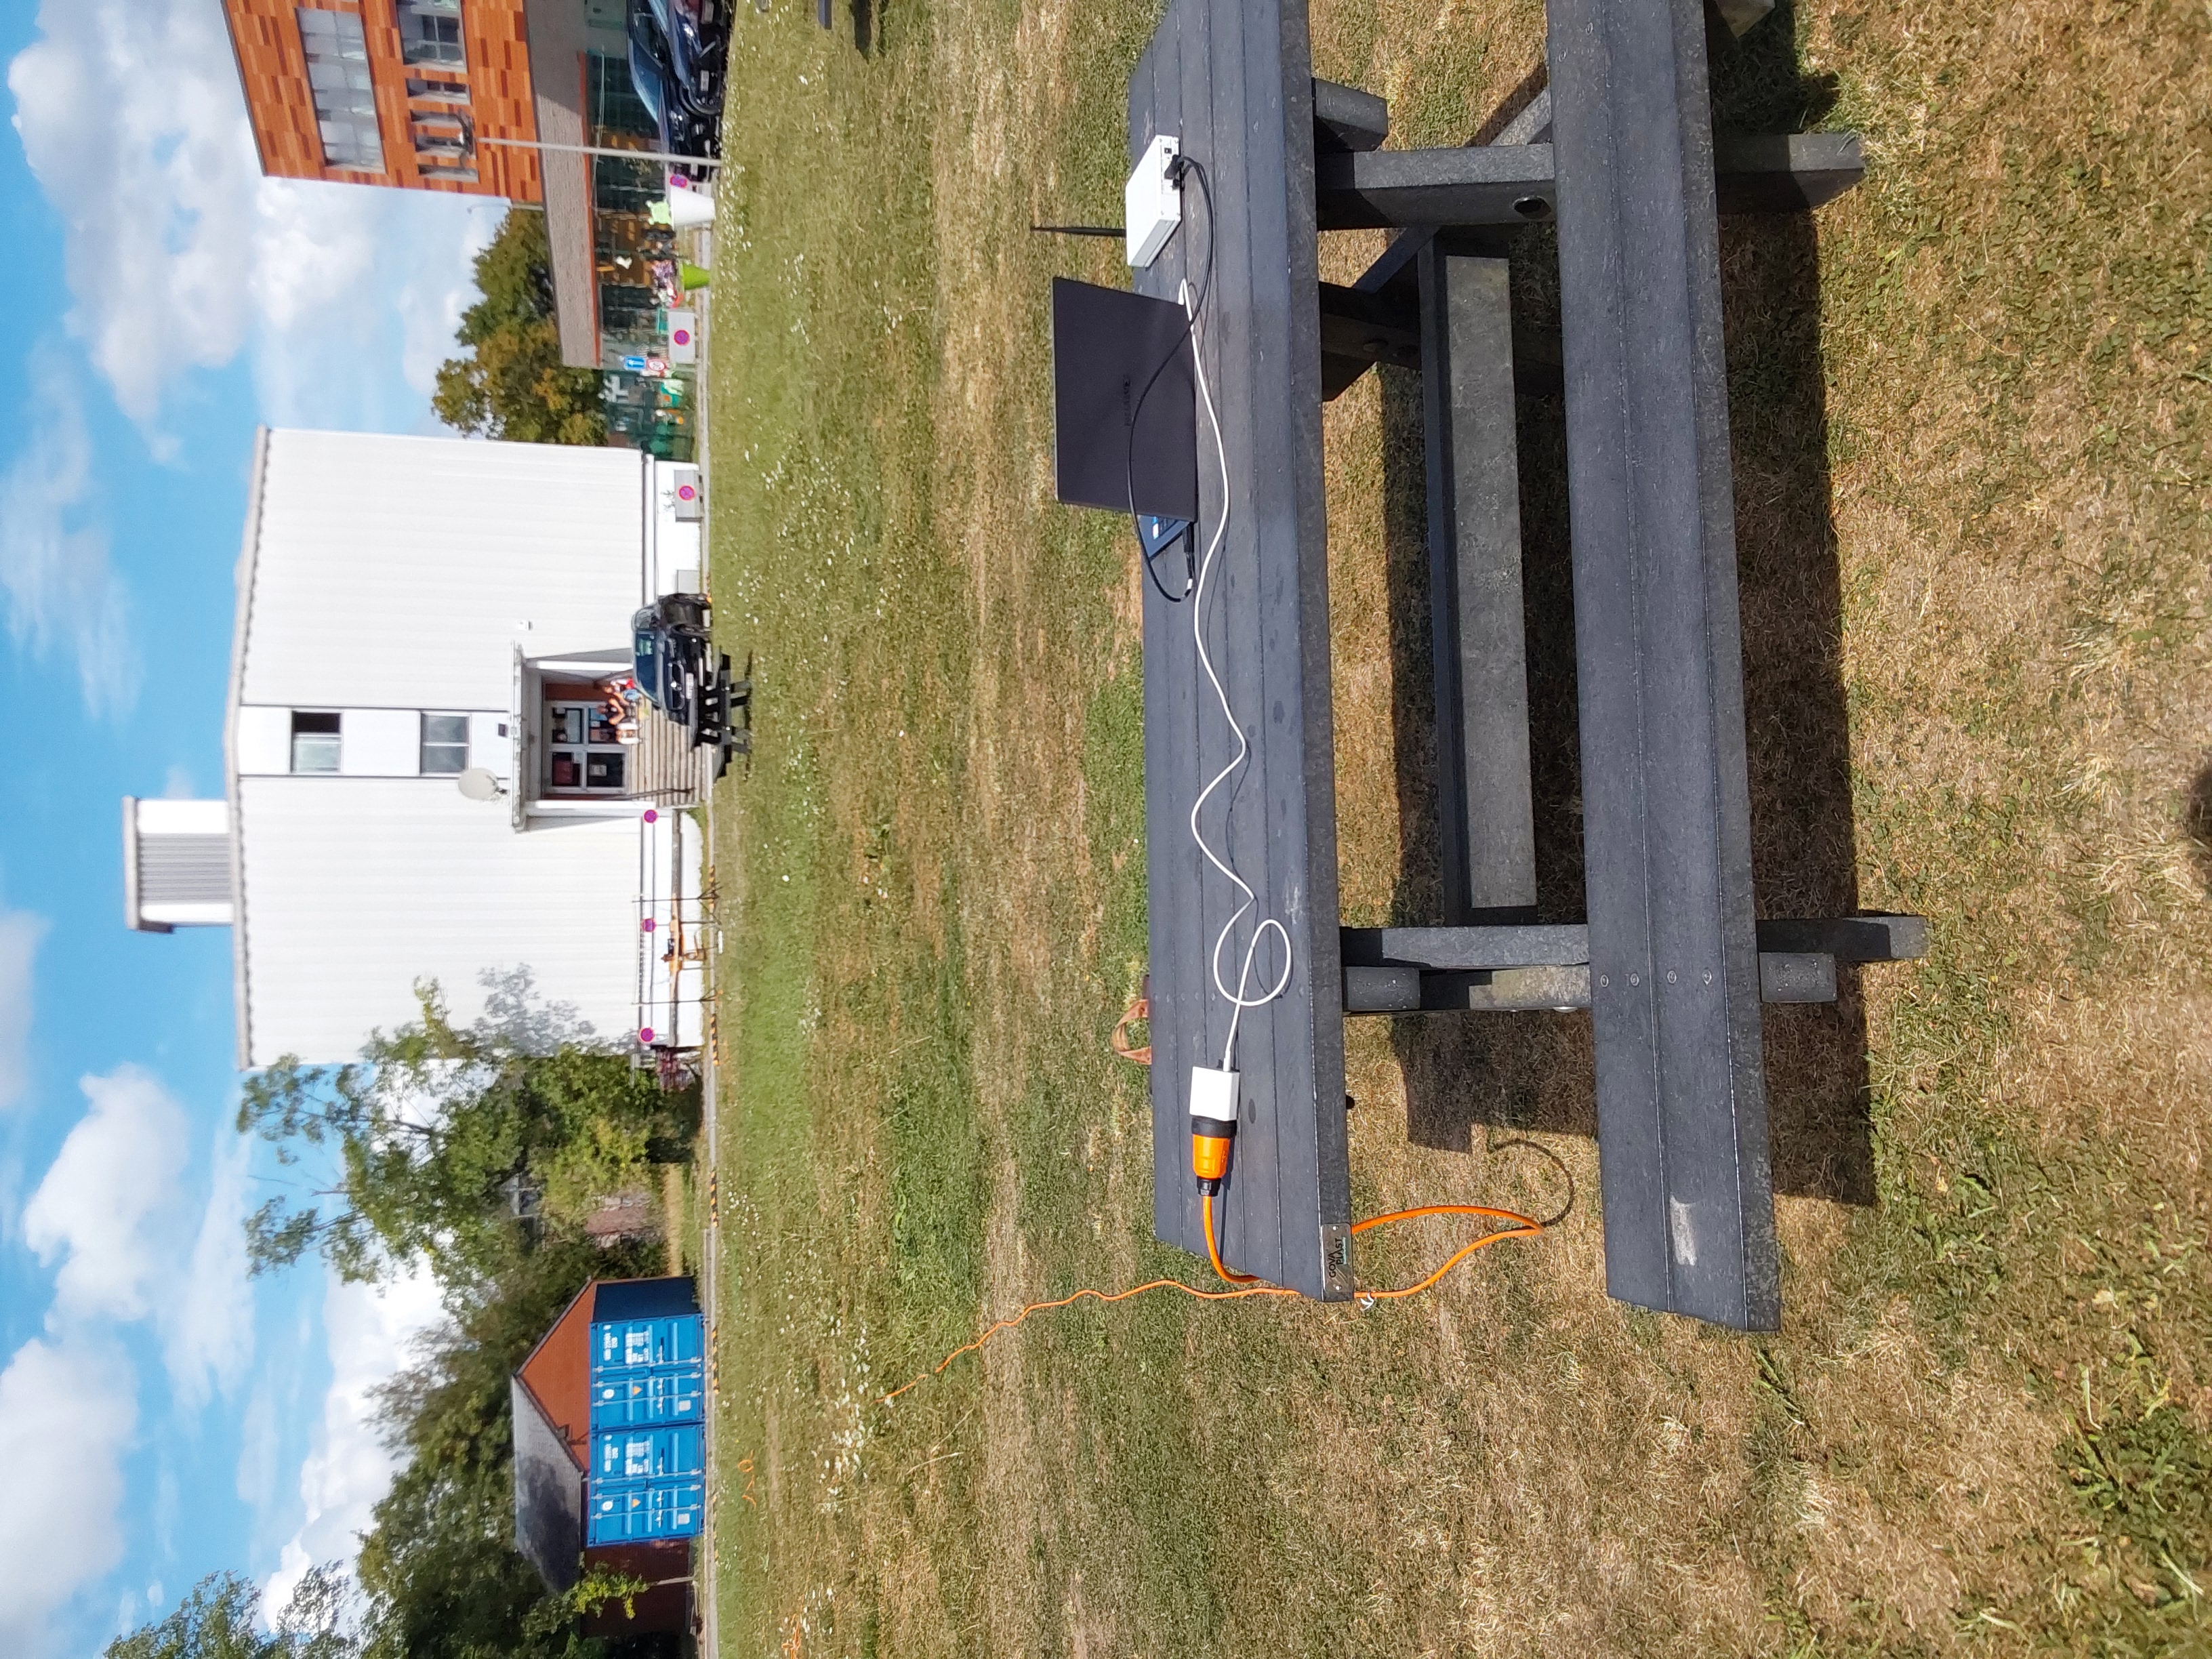
\includegraphics[width=\textwidth, angle=270]{figures/outside rx.jpg}
      \caption{Outdoors scenario}
    \end{subfigure}

    \caption{Receiver side indoors and outdoors}
    \end{adjustwidth}
  \end{figure}
\end{frame}



\subsection{Transmission methods}
\begin{frame}
  \frametitle{Transmission methods}
  \only<2>{
  \textbf{Round Robin (RR) }: each device sends a frame then passes the turn to the next one. The last device passes the turn to the first one. \\ }

  \only<3>{
  \textbf{One by One (ObO)}: each device sends all its frames then passes the turn to the next one.}

  \begin{figure}[ht]
  \begin{adjustwidth}{-10cm}{-10cm}
    \centering

  \only<2>{
    \begin{subfigure}[ht]{0.5\textwidth}
      \centering
      \includesvg[width=0.98\textwidth]{figures/RR.svg}
      \caption{RR method}
    \end{subfigure}
  }
  \only<3>{
    \begin{subfigure}[ht]{0.5\textwidth}
      \centering
      \includesvg[width=\textwidth]{figures/ObO.svg}
      \caption{ObO method}
    \end{subfigure}
  }
    \end{adjustwidth}
  \end{figure}

\end{frame}


\begin{frame}
  \frametitle{Comparison properties}
  The most important properties to compare those methods are :
  \begin{enumerate}
    \item Quality : How little the scheduling impacts the DL classification
    \item Safety : At any point, the receiver has to be certain of the origin of a LoRa frame
  \end{enumerate}

\end{frame}

\begin{frame}
  \frametitle{Selection}

  \only<2>{
  \begin{figure}
    \begin{center}
      \includesvg[width=0.90\textwidth]{figures/temp1.svg}
    \end{center}
  \end{figure}}

  \only<3>{
  \begin{figure}
    \begin{center}
      \includesvg[width=0.90\textwidth]{figures/temp2.svg}
    \end{center}
  \end{figure}}

  \only<4>{
  \begin{figure}
    \begin{center}
      \includesvg[width=0.90\textwidth]{figures/temp3.svg}
    \end{center}
  \end{figure}}

  \only<5>{
  \begin{figure}
    \begin{center}
      \includesvg[width=0.80\textwidth]{figures/temp3.svg}
    \end{center}
  \end{figure}}

  \only<5>{
  Even thought quality is an important property, safety is mandatory.\\ 
  \hspace{1cm}
   
  Because misclassification can occur when a device passes its turn, to avoid any misclassification by the receiver, the One by One method was selected. }
\end{frame}
  


